\documentclass[12pt,oneside,a4paper]{article}
%\documentclass{llncs}
\usepackage[utf8x]{inputenc}
\usepackage[T1]{fontenc}
\usepackage[english,polish]{babel}
\usepackage{polski}
\usepackage{float}
\usepackage{hyperref} %spis treści niech będzie łączami
\usepackage{listings}
\hypersetup{
	plainpages=false,
    colorlinks,
    citecolor=black,
    filecolor=black,
    linkcolor=black,
    urlcolor=black
}
\usepackage{graphicx}
\usepackage{pbox}
\usepackage{tabto}
\usepackage{algorithm}
\usepackage{algpseudocode}
% ustawienia środowiska algorytm
\floatname{algorithm}{Algorytm}
\renewcommand{\algorithmicfunction}{\textbf{funkcja}}
% koniec ustawień

% blokada dzielenia wyrazów (dla kopiowania do Worda)
% \hyphenpenalty 10000
% \exhyphenpenalty 10000
% koniec ustawień blokady

\begin{document}
\author{
  Jacek Sosnowski
  \and
  Michał Cybulski
}

\title{Implementacja i porównanie algorytmów CHARM i CLOSET}
\pagenumbering{alph}
\maketitle
%\input{tex/strona_tytulowa.tex}
\clearpage
\tableofcontents
\clearpage
\pagenumbering{arabic}

\section{Cel pracy}

Celem projektu jest implementacja obu algorytmów z wykorzystaniem języka Java w wersji 8.
Kolejnym kluczowym etapem będzie sprawdzenie poprawności obu implementacji.
Pozytywne zakończenie tego etapu pozwoli na wykonanie szeregu testów wydajnościowych służących analizie porównawczej obu algorytmów.
Naszym priorytetem jest sprawdzenie dwóch implementacji wykonanych we współczesnym języku programowania i znalezienie odpowiedzi na pytanie: które z tych dwóch podejść jest wydajniejsze?
Zamierzamy odnosić się również do wyników eksperymentów opisanych w pracach autorstwa J.Pei \cite{closetArt} w celu weryfikacji wniosków tam przedstawionych.


\section{Algorytm Charm}

Algorytm Charm opisany w artykule \cite{charmArt} służy do wyszukiwania wszystkich domkniętych zbiorów częstych w zbiorze danych transakcyjnych. Sposób jego działania pozwala na bardzo tanie pozbywanie się zbiorów redundantnych (i takich, które będą generowały redundantne zbiory), co w praktyce w bardzo dużym stopniu ogranicza złożoność obliczeniową potrzebną do wygenerowania zbiorów częstych. Algorytm został przedstawiony w pseudo-kodzie \ref{charmAlgorithm}.

\begin{algorithm}
\caption{Algorytm Charm}
\label{charmAlgorithm}
\renewcommand{\algorithmicrequire}{\textbf{Wejście:}}
\renewcommand{\algorithmicensure}{\textbf{Wyjście:}}
\begin{algorithmic}
	\Require Transakcyjna baza danych TDB i próg minimalnego wsparcia min\_sup.
	\Ensure  Kompletny zbiór częstych zbiorów domkniętych.
	\Function{charm}{$TDB \subseteq \mathcal{I} \times \mathcal{T}$, $min\_sup$}
		\State $nodes \gets \{I_{j} \times t(I_{j}) : I_{j} \in \mathcal{I} \wedge |t(I_{j})| \ge min\_sup \} $
		\State $FCI \gets \emptyset$ \Comment{$FCI$ to zbiór częstych zbiorów zamkniętych}
		\State $\Call{charmExtend}{nodes, FCI}$
		\State \Return $FCI$
	\EndFunction
	\Function{charmExtend}{$nodes$, $FCI$}
		\ForAll {$X_{i} \times t(X_{i}) \in nodes$}
			\State $newN \gets \emptyset$
			\State $X = X_{i}$
			\ForAll {$ X_{j} \times t(X_{j}) \in nodes : f(j) > f(i) $} \Comment{$f(a)$ - funkcja ustalająca kolejność (np. wg kolejności leksykalnej lub wsparcia)}
				\State $X = X \cup X_{j}$
				\State $Y = t(X_{i}) \cap t(X_{j})$
				\State $\Call{charmProperty}{nodes, newN}$
			\EndFor
			\If {$newN \neq \emptyset $}
				\State $\Call{charmExtend}{newN, FCI}$
			\EndIf
		\EndFor
	\EndFunction
	\Function{charmProperty}{$nodes, newN$}
		\If{$|Y| > min\_sup$}
			\If{$t(X_{i}) = t(X_{j})$}
				\State Remove $X_{j}$ from $nodes$
				\State Replace all $X_{i}$ with $X$
			\ElsIf{$t(X_{i}) \subset t(X_{j})$}
				\State Replace all $X_{i}$ with $X$
			\ElsIf{$t(X_{i}) \supset t(X_{j})$}
				\State Remove $X_{j}$ from $nodes$
				\State Add $X \times Y$ to $newN$
			\ElsIf{$t(X_{i}) \neq t(X_{j})$}
				\State Add $X \times Y$ to $newN$
			\EndIf
		\EndIf
	\EndFunction
\end{algorithmic}
\end{algorithm}

Cechą wyróżniającą algorytm Charm jest to, że algorytm ten działa praktycznie jednocześnie zarówno na przestrzeni elementów jak i na przestrzeni identyfikatorów transakcji, podczas gdy większość algorytmów porusza się wyłącznie po przestrzeni elementów. Ta cecha pozwala na wykorzystanie bardzo efektywnej metody badania czy rozpatrywany zbiór jest zbiorem domkniętym i ignorowanie go w przeciwnym wypadku. Analizowane zbiory nie są więc eliminowane tylko na podstawie małej częstości ich występowania, ale także na podstawie braku ich domknięcia.

Algorytm Charm nie korzysta w swojej implementacji z drzew, jak typowe algorytmy generujące zbiory częste. Autorzy sugerują natomiast, żeby dane trzymać w postaci ,,pionowej'' (ang. ,,vertical data format''), czyli niejako przyporządkowując każdemu elementowi zbiór identyfikatorów transakcji, w których on występuje. Dzięki temu operacje sumy oraz przecięć zbiorów oraz wykrywanie czy zbiór transakcji jednego elementu zawiera się w zbiorze drugiego elementu (lub vice versa) są bardzo tanie (praktycznie darmowe) -- zwłaszcza w porównaniu z sytuacją, gdy dane trzymane są standardowo, czyli zbiory elementów przyporządkowywane są poszczególnym transakcjom, a takie porównanie oznacza konieczność iteracji po wszystkich transakcjach.

\section{Algorytm Closet}

Algorytm Closet oparty jest na idei ,,dziel i zwyciężaj''. 
Z tego powodu zbiór danych transakcyjnych (oznaczany w oryginalnym artykule jako TDB -- transakcyjna baza danych) dzielony jest rekurencyjnie na mniejsze podzbiory. Wykonywane jest to z uwzględnieniem znalezionych na danym poziomie zbiorów częstych.

Zamiast operacji bezpośrednio na strukturze transakcyjnej autorzy zalecają bezpośrednią pracę na drzewie FP-tree. 
Jest to drzewo prefiksowe reprezentujące skompresowany ale kompletny zestaw zbiorów częstych w dostępnej bazie danych.

Sam algorytm Closet (nawiązując do artykułu \cite{closetArt}) można przedstawić ogólnie w pseudokodzie -- Algorytm \ref{closetAlgorithm}.

\begin{algorithm}
\caption{Algorytm Closet}
\label{closetAlgorithm}
\renewcommand{\algorithmicrequire}{\textbf{Wejście:}}
\renewcommand{\algorithmicensure}{\textbf{Wyjście:}}
\begin{algorithmic}
	\Require Transakcyjna baza danych TDB i próg minimalnego wsparcia min\_sup.
	\Ensure  Kompletny zbiór częstych zbiorów domkniętych.
	\Function{AlgorytmCloset}{} 
		\State $FCI \gets \emptyset$ \Comment{$FCI$ to zbiór zbiorów zamkniętych}
		\State $f\_list \gets \Call{ZnajdzZbioryCzęste}{TBD}$ \Comment{f\_list - lista zb. częstych}
		\State \Return \Call{Closet}{$\emptyset, TBD, 	f\_list, FCI$}
	\EndFunction
\end{algorithmic}
\end{algorithm}

Natomiast użyta tam procedura \textit{Closet(X, DB, f\_list, FCI)} wykonuje kilka kroków: 

\begin{enumerate}
  \item (Optymalizacja nr 2 z pracy \cite{closetArt}). Niech $Y$ zawiera te elementy $f\_list$, które występują w każdej transakcji z DB, wstaw $X \cup Y$ do $FCI$ z takim samym wsparciem.
  \item Zbuduj drzewo FP-tree dla danego DB.
  \item (Optymalizacja nr 3 z pracy \cite{closetArt} -- wydobycie częstych zbiorów zamkniętych $iX$, jeśli możliwe.
  \item Formacja warunkowej bazy danych $DB|i$ dla każdego elementu $i$ z	 $f\_list$, obliczenie zbiorów częstych (zwykłych). 
  \item Dla każdego elementu $i$ z $f\_list$ należy rekurencyjnie wywołać funkcję \textit{Closet(iX, DB|i, f\_list|i, FCI)}.
\end{enumerate}

Implementacja pełnego algorytmu wymaga podjęcia decyzji odnośnie struktur danych, które będą użyte. 
Jak już było wspomniane wcześniej -- autorzy zalecają wykorzystanie drzewa FP-tree. 
Jednak dla bardzo dużych baz danych problemem staje się operowanie taką strukturą w pamięci operacyjnej komputera. 
Pierwszym rozwiązaniem jest implementacja korzystająca z pamięci dyskowej.
Drugim częściowe reużycie fragmentów drzewa (ang. partition-based approach).
W kontekście naszej pracy oba podejścia mają wady. Pierwsze w postaci opóźnień przy dostępie do wywołań systemowych (operacje dyskowe). Stanowią one znaczący narzut, który nie podlega bezpośredniej kontroli.
Drugie podejście tworzy skomplikowaną strukturę, wymagającą transferu transakcji pomiędzy warunkowymi bazami danych na danym poziomie rekurencji. 
Jej użycie wiązałoby się z koniecznością ewaluacji wydajności samej struktury i samego algorytmu oddzielnie.
Z racji, że jedynym celem jest ocena wyłącznie samego algorytmu, wynika że dołączanie do niego skomplikowanej struktury utrudni wszelkie obserwacje jego zachowania (przede wszystkim pomiary).
Dlatego tymczasowym i wstępnym założeniem, niech będzie fakt, niewykorzystywania bardzo dużych zbiorów danych, które wymagałyby angażowania, któregoś z powyższych rozwiązań i pozostanie przy standardowym wykorzystaniu drzewa FP-tree.



\section{Realizacja projektu}

\subsection{Implementacja}

Implementacje obu algorytmów to oddzielne aplikacje konsolowe napisane w języku Java 8. Każdy z członków zespołu zajął się implementacją jednego z algorytmów, co pozwoliło na zrównoleglenie pracy. Do budowania aplikacji wykorzystano \emph{Gradle}.

Implementując oba algorytmy nie korzystano z żadnych dodatkowych bibliotek wykonujących istotną część zadania -- wykorzystano natomiast szereg bibliotek pomocniczych:

\begin{itemize}
	\item \emph{Open CSV} -- do obsługi wczytywania danych z plików \emph{CSV}
	\item \emph{Logback} -- obsługa logowania
	\item \emph{Google Guava}, \emph{Apache Commons} -- rozmaite narzędzia ,,utility''
	\item \emph{JUnit}, \emph{AssertJ} -- testy jednostkowe
\end{itemize}

\subsection{Budowanie aplikacji}

Obie aplikacje można wygodnie zbudować za pomocą systemu \emph{Gradle}. Komendy:
\begin{lstlisting}
./gradlew clean
./gradlew build
\end{lstlisting}

W wyniku wywołania komend w katalogach $build/lib/$ pojawią się wykonywalne pliki Java z rozszerzeniem $*.jar$.

\subsection{Uruchamianie}


Oba stworzone w ramach projektu programy można uruchomić z poziomu konsoli.

Dane wejściowe, na których testowane były algorytmy pochodziły z repozytorium UCI \cite{UCI} -- zbiór danych to ,,\emph{Mushroom Database}''. Zbiór ten zawiera dane o 8124 grzybach, z których każdy opisany jest 22 atrybutami.

\begin{itemize}
  \item Obie implementacje będą oddzielnymi aplikacjami konsolowymi.
  \item Językiem programowania będzie Java 8.
  \item System budowania opierać się będzie o technologię Gradle.
  \item Dane wejściowe będą stanowić zbiory danych z repozytorium UCI \cite{UCI}.
  \item Dane wyjściowe będą wyprowadzane na standardowe wyjście lub do pliku.
  \item Wszelkie użycia dodatkowych bibliotek nie będą związane z główną funkcjonalnością programów, a jedynie z funkcjami pomocniczymi (np. z logowaniem, czy z testowaniem aplikacji).
\end{itemize}


\section{Testy}

TODO -- proszę uzupełnić.

\subsection{Profilowanie}

\subsubsection{CHARM}

Wyniki profilowania algorytmu CHARM znajdują się na Rys. \ref{charm:profil}. Tak jak można było się spodziewać, większość czasu program spędził w głównej metodzie algorytmu. Można zauważyć, że aż 10\% czasu procesora zostało zużyte na wyliczanie funkcji skrótu obiektów. Wynika to z tego, że w algorytmie występuje bardzo dużo porównywania zbiorów transakcji, w których występują poszukiwane zbiory częste. Jako, że najszybsze wyszukiwanie w tego typu warunkach gwarantowały kolekcje \emph{HashSet}, to one zostały wykorzystane w tych kluczowych miejscach. Na dole wykresu widać także, że wykorzystanie 13\% czasu procesora związane było z obsługą wielowątkowości. Pomimo nie napisania żadnego specjalnego kodu do obsługi wielu wątków dzięki wykorzystaniu mechanizmu \emph{parallelStream}, który pojawił się w Java 8, w bardzo prosty sposób można zrównoleglić niektóre operacje na kolekcjach, co zostało wykorzystane w projekcie.

\begin{figure}
\caption{Wyniki profilowania algorytmu CHARM}
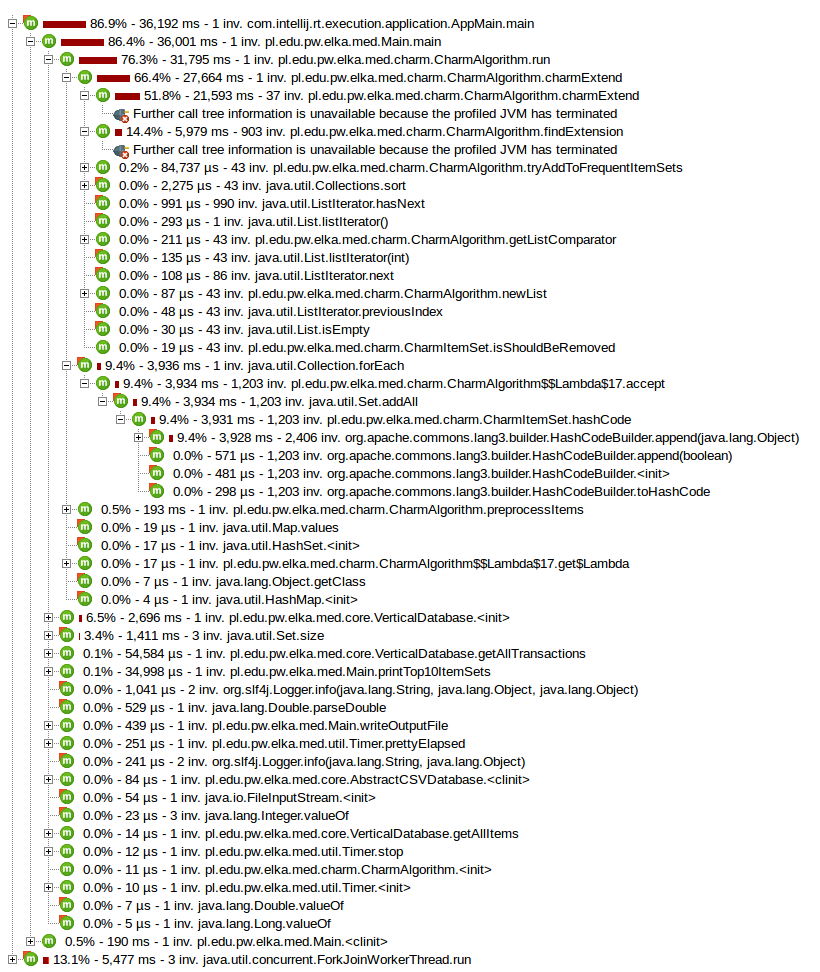
\includegraphics[width=17cm]{res/charm-profi.png}
\label{charm:profil}
\end{figure}

\subsubsection{CLOSET}

TODO -- proszę opisać trochę jakieś ewentualne obserwacje. Wyniki profilowania algorytmu CHARM znajdują się na Rys. \ref{closet:profil}.

\begin{figure}
\caption{Wyniki profilowania algorytmu CHARM}
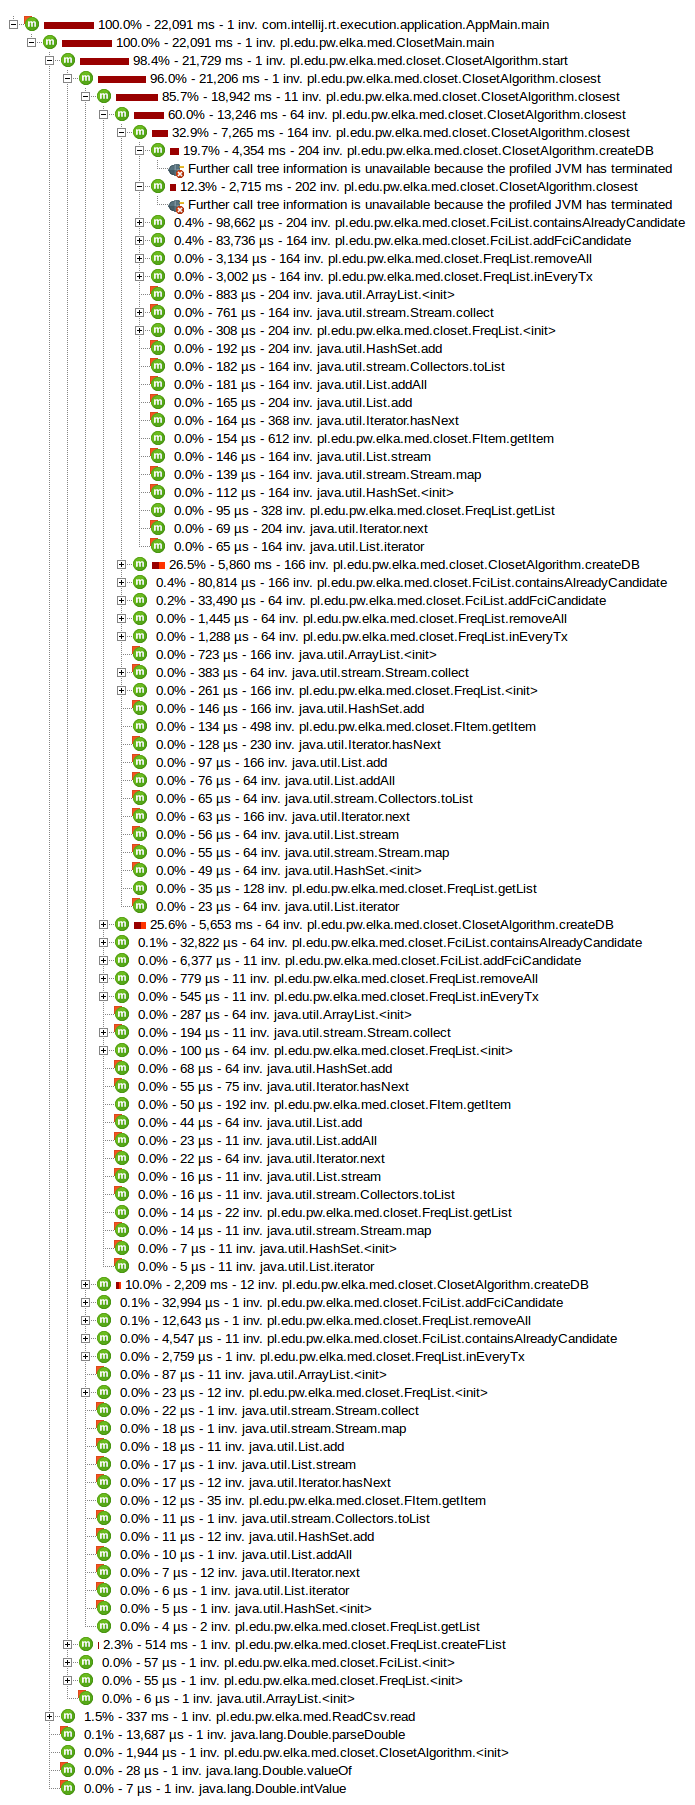
\includegraphics[width=14cm]{res/closet-profi.png}
\label{charm:profil}
\end{figure}

\clearpage
\bibliographystyle{splncs}
\begin{thebibliography}{99}

\bibitem{charmArt} \emph{CHARM: An Efficient Algorithm for Closed Association Rule Mining}, Mohammed J. Zaki, Ching-Jui Hsiao, 2005

\bibitem{closetArt} \emph{CLOSET: An Efficient Algorithm for Mining Frequent Closed Itemsets}, Jian Pei, Jiawei Han, Runying Mao, 2000


\end{thebibliography}

\end{document}
